\section{Anwendung}
\subsection{Projekt erstellen}
\subsubsection{Git-Repo initialisieren}

\subsubsection{Dateistruktur}
Abbildung \ref{fig:OrdnerDatei} zeigt die empfohlene Ordner und Dateistruktur für neue Projekte am Beispiel des "`HowTo"'-Projektes.
Die Ordner "`tikz"' und "`idiotenseite"' müssen natürlich nur erstellt werden wenn sie auch gebraucht werden. In allen Ordnernamen werden nur
Kleinbuchstaben verwendet, die einzige Ausnahme bildet der Hauptordner, welcher gleich benannt wird wie das offizielle Modulkürzel des Faches.
Die Hauptdatei (das ist diejenige in der \verb+\begin{document}+ \ldots \verb+\end{document}+ steht) wird ebenfalls nach dem Modulkürzel benannt.
Die einzelnen Kapitel (\verb+\section{}+) werden im Ordner \verb+sections+ abgelegt und nachher mit \verb+\input{}+ in das Hauptdokument eingebunden.
Der Dateiname sollte möglichst dem Titel des Kapitels entsprechen. Bilder und Grafiken welche mit externen Programmen erstellt wurden sind im Ordner
\verb+images+ abzulegen. Alles was zur Konfiguration des Layouts dient findet den Platz im \verb+header+ Ordner, TikZ-Grafiken werden im entsprechenden
\verb+tikz+ Ordner abgelegt.

\begin{figure}[h]
\begin{center}
  \begin{tikzpicture}[%
	grow via three points={one child at (0.5, -0.8) and
	two children at(0.5,-0.8) and (0.5, -1.6)},
	edge from parent path={(\tikzparentnode.south) |- (\tikzchildnode.west)}]
	\tikzstyle{every node}=[anchor=west, minimum width=2.5cm, minimum height=0.6cm]
	\tikzstyle{folder}=[draw=black, thick]
	\tikzstyle{optional}=[dashed, folder]
	\node[folder] {HowTo}
		child {node[folder] {header}}
		child {node[folder] {sections}}
		child {node[folder] {images}}
		child {node[optional] {tikz}}
		child {node[optional] {idiotenseite}}
		child {node {HowTo.tex}};
  \end{tikzpicture}
  \caption[Ordner und Dateistruktur]{Ordner und Dateistruktur für neue Projekte}
  \label{fig:OrdnerDatei}
\end{center}
\end{figure}

Weitere Dateien im Hauptverzeichnis, welche in Abbildung \ref{fig:OrdnerDatei} nicht ersichtlich sind:
\begin{description}
  \item[README.md] Hier kommt eine kurze Beschreibung des Projekts hin. Bei Zusammenfassungen ist es sinnvoll den Dozenten zu erwähnen,
  	bei dem die Vorlesung stattgefunden hat.
  \item[.gitignore] Gitignore-Datei mit den relevanten Einträgen
  \item[Makefile]	Falls ein Makefile verwendet wird
\end{description}

\subsubsection{Dateivorlagen}


\subsection{Code Snippets}
Das Listings\footnote{\url{http://www.ctan.org/pkg/listings}} Paket bietet Support für über 80 Programmiersprachen, dazu kommen für verschiedene Sprachen noch diverse Dialekte. Sollte das nicht
ausreichen lässt sich relativ leicht eine neue Sprache definieren.

Als Beispiel hier der (gekürzte) TikZ-Code für Abbildung \ref{fig:OrdnerDatei}:
\lstset{language=[LaTeX]TeX,
	morekeywords={node, child, tikzstyle}
}
\begin{lstlisting}
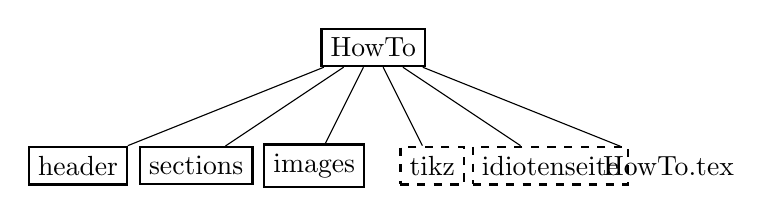
\begin{tikzpicture}
  \tikzstyle{folder}=[draw=black, thick]
  \tikzstyle{optional}=[dashed, folder]
  \node[folder] {HowTo}
    child {node[folder] {header}}
    child {node[folder] {sections}}
    child {node[folder] {images}}
    child {node[optional] {tikz}}
    child {node[optional] {idiotenseite}}
    child {node {HowTo.tex}};
\end{tikzpicture}
\end{lstlisting}


\subsubsection{Aufzählungen}
http://www.ctan.org/pkg/enumitem

\subsubsection{Bilder}
Zum Bilder einfügen: http://www.ctan.org/tex-archive/macros/latex/required/graphics/ \\
Bilder in Tabellen: http://www.ctan.org/pkg/adjustbox

\subsubsection{Grafiken (TIKZ)}
http://www.ctan.org/pkg/pgf

\subsubsection{mehrere Spalten}
http://www.ctan.org/pkg/multicol


\subsubsection{Formeln}
\subsubsection{Tabellen}
http://www.ctan.org/pkg/tabularx